\documentclass[a4paper]{article}

\title{Protein HMM}
\author{Danilo Horta}
\date{August 2019}

\usepackage{natbib}
\usepackage{graphicx}
\usepackage{amsmath}
\usepackage{amsthm}
\usepackage[margin=0.5in]{geometry}
\usepackage{rotating}

\theoremstyle{definition}
\newtheorem{example}{Example}[section]

\theoremstyle{definition}
\newtheorem{definition}{Definition}[section]

\newcommand{\prob}[1]{p (#1)}
\newcommand{\cprob}[2]{p\left(#1\;\middle|\; #2\right)}
\newcommand{\eps}{\epsilon}
\newcommand{\s}{\texttt{\char`_}}

\begin{document}

\maketitle

\section{Model}

\begin{definition}
Let $\mathcal A$ be the alphabet of amino acids.
Let $Q_1, Q_2, \dots$ be a Markov process with (possibly) silent states and let $S_1, S_2, \dots$ be a stochastic process for which
$\cprob{S_i\in\mathcal A}{Q_1=q_1, Q_2=q_2, \dots} = \cprob{S_i\in\mathcal A}{Q_t=q_t}$ for some $t$.
The pair $(Q_t, S_i)$ is a hidden Markov model with (possibly) silent states (HMM) and alphabet $\mathcal A$.
\end{definition}

Let $(Q_t, S_i)$ be an amino acid HMM with alphabet $\mathcal A$.
We want to replace it with a HMM that generates sequences of symbols from the alphabet
$\mathcal B = \{\mathrm A, \mathrm C, \mathrm G, \mathrm T\}$ of DNA bases and is able to account
for frame-shifting.
Let $\mathrm M_j$ be the so-called match state of an amino acid HMM and let $Q_t=\mathrm M_j$.
From the amino acid emission probabilities and any other relevant source of information
(codon usage bias, for instance), one can define the probability $\cprob{X_1=x_1, X_2=x_2, X_3=x_3}{Q_t=\mathrm M_j}$
of $\mathrm M_j$ emitting the codon $(x_1, x_2, x_3) \in \mathcal B^3$
--- one can also write $\cprob{X=x_1x_2x_3}{Q_t=\mathrm M_j}$, for short.
Since measurement errors occur and nature is not perfect, we will replace the
codon emission process by one that instead produces base sequences of different
lengths to account for base insertions and deletions (indels).

Node $\mathrm M_j$ in Fig.~\ref{fig:codon-hmm-tree} represents the modified match state.
The generated codon will go through four transitions, each one representing one of three possibilities: (i) delete a base; (ii) insert a base; or (iii) do nothing.
The deletion can happen in any of the three codon positions with equal probability.
If a deletion has already happened, the next deletion can happen in any of the remaining two positions with equal probability.
The insertion can happen between any two bases, before the first base or after the last base with equal probability.

\begin{sidewaysfigure}[ht]
    \centering
    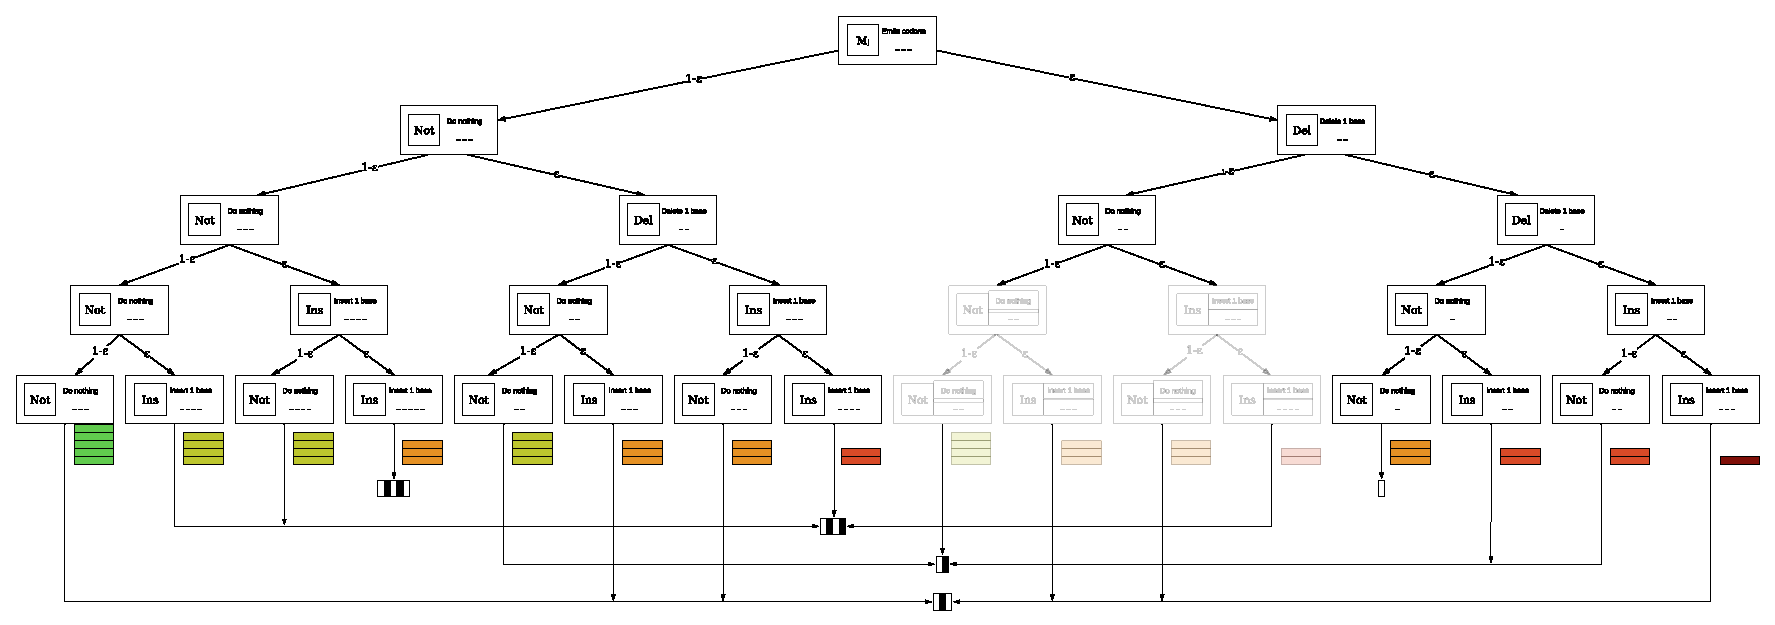
\includegraphics[scale=0.9]{codon-hmm-tree}
    \caption{Matched codon HMM tree.
        The $\eps$-transitions occur infrequently and exist to account for sequence errors.
        The most probably path ends at the first leaf-node from left to right.}\label{fig:codon-hmm-tree}
\end{sidewaysfigure}

There are five likelihood levels for paths starting at node $\mathrm M_j$ and ending at some leaf-node in Fig.~\ref{fig:codon-hmm-tree}.
Let $l\in\{0, 1, 2, 3, 4\}$ represent different likelihood levels such that $p(l=4)$ denotes the probability of
the most probable paths, $l=3$ denotes the probability of the second most probable paths, and so forth.
We have
\begin{align*}
    p(l) = \binom{4}{l} (1 - \eps)^{l}\eps^{4-l},
\end{align*}
where coefficient $\binom{4}{l}$ counts the number of paths corresponding to level $l$.
Let $F$ be a random variable representing the final sequence length generated by the model in
Fig.~\ref{fig:codon-hmm-tree}.
We have
\begin{align*}
    p(Z=1) = p(Z=5) &= \eps^2(1-\eps)^2, \\
    p(Z=2) = p(Z=4) &= 2\eps^3(1-\eps) + 2\eps(1-\eps)^3,~\text{and} \\
    p(Z=3)          &= \eps^4 + 4\eps^2(1-\eps)^2 + (1-\eps)^4.
\end{align*}
Fig.~\ref{fig:seq-len-prob} shows the sequence length distributions over different values of $\eps$.

\begin{figure}[htbp]
\centering
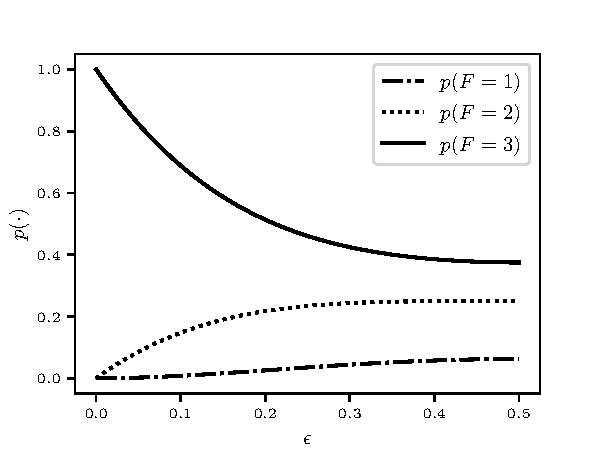
\includegraphics[scale=0.25]{seq-len-prob}
\caption{Sequence length distributions over $\eps$.}\label{fig:seq-len-prob}
\end{figure}

A sequence $\mathbf z=z_i z_{i+1}\dots$ of finite but variable length will emerge at the end of the process represented in Fig.~\ref{fig:codon-hmm-tree}.

Let $\mathcal Q_f$ be the set of hidden paths, starting with $Q_t=\mathrm M_j$ and ending with $Q_{t+4}$,
that generate sequences of length $f$.
Let $Z=(Z_i, \dots, Z_{i+f-1})$.
We have
\begin{align*}
    \cprob{Z=z_1,\dots,z_f,F=f}{Q_t=\mathrm M_j} &= \sum_{\mathbf q \in \mathcal Q_f}
            \cprob{Z_i=z_1,\dots,Z_{i+f-1}=z_f}{Q_t=\mathrm M_j, Q=\mathbf q}\\
        &\times\cprob{Q=\mathbf q}{Q_t=\mathrm M_j}.
\end{align*}

\section{Emission probabilities}

\begin{align*}
    \cprob{Z=z_1,F=1}{\mathrm M_j}
        &= \eps^2(1-\eps)^2(p(X=z_1\s\s) + p(X=\s z_1\s) + p(X=\s\s z_1)) / 3
\end{align*}

\begin{align*}
    \cprob{Z=z_1z_2,F=2}{\mathrm M_j}
        &= 2\eps(1-\eps)^3(p(X=\s z_1z_2) + p(X=z_1\s z_2) + p(X=z_1z_2\s))/3\\
        &+ \eps^3(1-\eps)(p(X=z_1\s\s) + p(X=\s z_1\s) + p(X=\s\s z_1))p(z_2)/3\\
        &+ \eps^3(1-\eps)(p(X=z_2\s\s) + p(X=\s z_2\s) + p(X=\s\s z_2))p(z_1)/3
\end{align*}


\begin{align*}
    \cprob{Z=z_1z_2z_3,F=3}{Q_t=\mathrm M_j} &= (1-\eps)^4 p(X=z_1z_2z_3)\\
        &+ 4\eps^2(1-\eps)^2 (p(X=\s z_2 z_3) + p(X=z_2\s z_3) + p(X=z_2 z_3\s))p(z_1)/9\\
        &+ 4\eps^2(1-\eps)^2 (p(X=\s z_1 z_3) + p(X=z_1\s z_3) + p(X=z_1 z_3\s))p(z_2)/9\\
        &+ 4\eps^2(1-\eps)^2 (p(X=\s z_1 z_2) + p(X=z_1\s z_2) + p(X=z_1 z_2\s))p(z_3)/9\\
        &+ \eps^4 (p(X=z_3\s\s) + p(X=\s z_3\s) + p(X=\s\s z_3))p(z_1)p(z_2)/9\\
        &+ \eps^4 (p(X=z_2\s\s) + p(X=\s z_2\s) + p(X=\s\s z_2))p(z_1)p(z_3)/9\\
        &+ \eps^4 (p(X=z_1\s\s) + p(X=\s z_1\s) + p(X=\s\s z_1))p(z_2)p(z_3)/9
\end{align*}

\begin{align*}
    \cprob{Z=z_1z_2z_3z_4,F=4}{Q_t=\mathrm M_j} &= \eps(1-\eps)^3 (p(X=z_2z_3z_4)p(z_1)+p(X=z_1z_3z_4)p(z_2)\\
    &+p(X=z_1z_2z_4)p(z_3)+p(X=z_1z_2z_3)p(z_4))/2\\
    &+2\eps^3(1-\eps)(\\
    &+p(X=\s z_3z_4)p(z_1)p(z_2) + p(X=\s z_2z_4)p(z_1)p(z_3)\\
    &+ p(X=\s z_2z_3)p(z_1)p(z_4) + p(X=\s z_1z_4)p(z_2)p(z_3)\\
    &+ p(X=\s z_1z_3)p(z_2)p(z_4) + p(X=\s z_1z_2)p(z_3)p(z_4)\\
    &+ p(X=z_3\s z_4)p(z_1)p(z_2) + p(X=z_2\s z_4)p(z_1)p(z_3)\\
    &+ p(X=z_2\s z_3)p(z_1)p(z_4) + p(X=z_1\s z_4)p(z_2)p(z_3)\\
    &+ p(X=z_1\s z_3)p(z_2)p(z_4) + p(X=z_1\s z_2)p(z_3)p(z_4)\\
    &+ p(X=z_3z_4\s)p(z_1)p(z_2) + p(X=z_2z_4\s)p(z_1)p(z_3)\\
    &+ p(X=z_2z_3\s)p(z_1)p(z_4) + p(X=z_1z_4\s)p(z_2)p(z_3)\\
    &+ p(X=z_1z_3\s)p(z_2)p(z_4) + p(X=z_1z_2\s)p(z_3)p(z_4))/9
\end{align*}

\begin{align*}
    \cprob{Z=z_1z_2z_3z_4z_5,F=5}{Q_t=\mathrm M_j}
        &= \eps^2(1-\eps)^2(\\
        &+p(z_1)p(z_2)p(X=z_3z_4z_5)+p(z_1)p(z_3)p(X=z_2z_4z_5)\\
        &+p(z_1)p(z_4)p(X=z_2z_3z_5)+p(z_1)p(z_5)p(X=z_2z_3z_4)\\
        &+p(z_2)p(z_3)p(X=z_1z_4z_5)+p(z_2)p(z_4)p(X=z_1z_3z_5)\\
        &+p(z_2)p(z_5)p(X=z_1z_3z_4)+p(z_3)p(z_4)p(X=z_1z_2z_5)\\
        &+p(z_3)p(z_5)p(X=z_1z_2z_4)+p(z_4)p(z_5)p(X=z_1z_2z_3))/10
\end{align*}

\end{document}
